%!TEX root = featurematch.tex
\subsection{Coarse-level Matching}
\label{ssec:methodology:naive}

For palmprint recognition, we need a measurement of similarity between two samples. If the similarity is high, we have a high confidence to believe that the two samples are from the same person. Otherwise we reject to claim that.

After mapping the high-dimensional feature vector to $\Gamma$-dimensional vector $\tilde{F}$, the similarity between two samples can be calculated as

\begin{equation}
Similarity= \| \tilde{F}_1 -\tilde{F}_2 \|
= \sum \limits_{i=1}^{\Gamma} (f_i^1-f_i^2)^2
\label{eq:methodology:similarity}
\end{equation}

\begin{figure}[htb]
  \begin{center}
    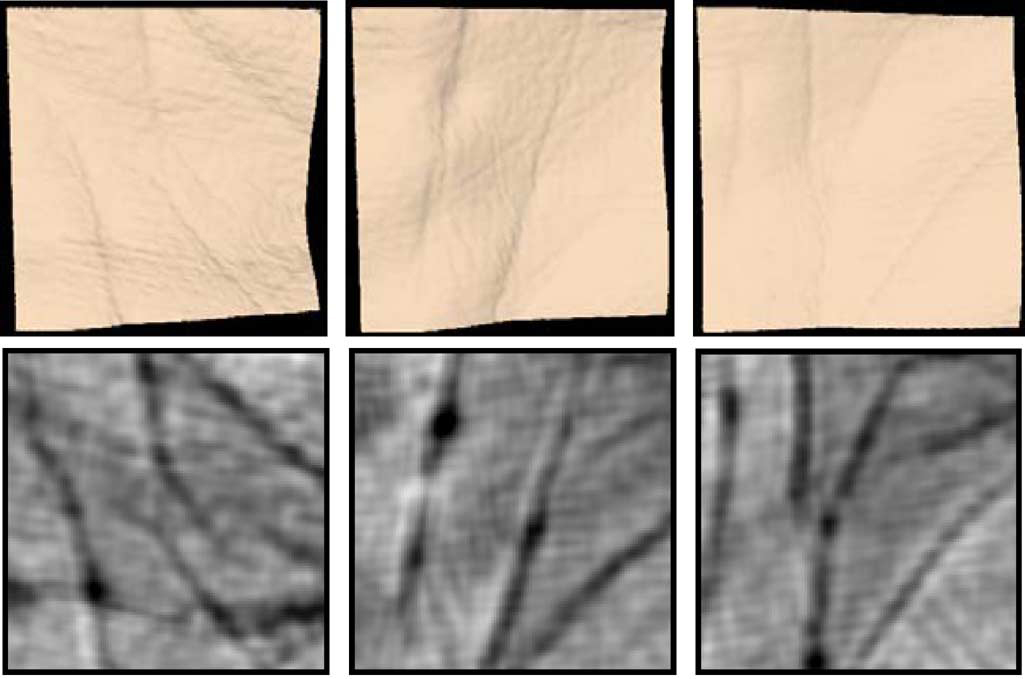
\includegraphics[width=0.9\linewidth]{ch-methodology/figures/mci1}
    \caption[MCI for ROIs from different palms]{Mean Curvature Image for ROIs from three different palms}    \label{fig:methodology:mci1}
  \end{center}
\end{figure}

\begin{figure}[htb]
  \begin{center}
    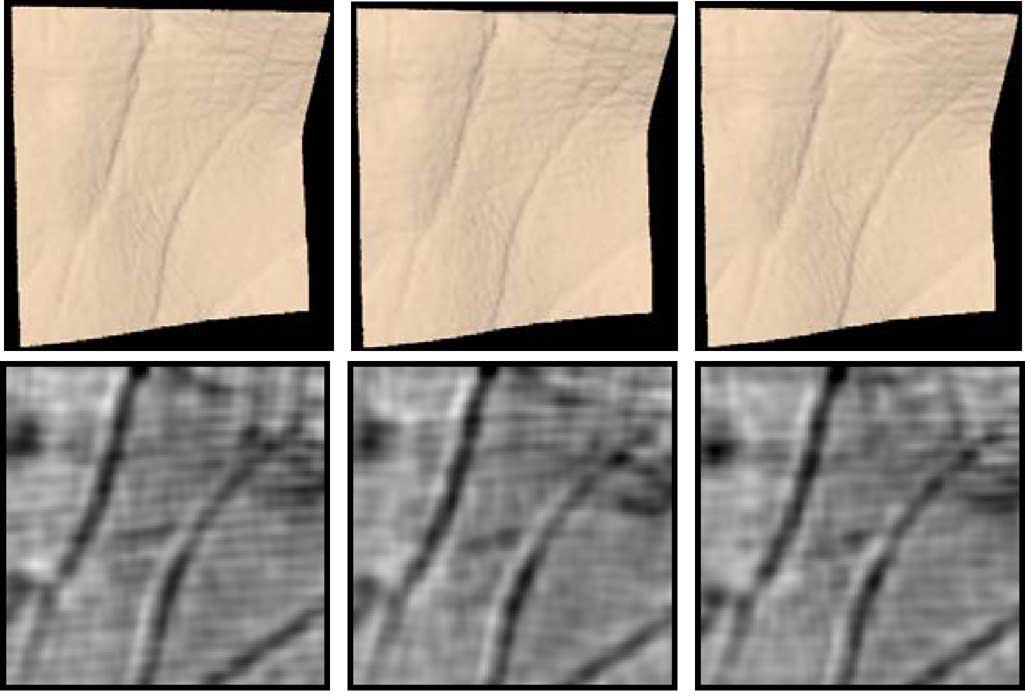
\includegraphics[width=0.9\linewidth]{ch-methodology/figures/mci2}
    \caption[MCI for ROIs from the same palm]{Mean Curvature Image for ROIs from three samples of the same palm}    \label{fig:methodology:mci2}
  \end{center}
\end{figure}

There are other features extracted from the same dataset such as Mean Curvature Image in ~\cite{Zhang:2009dp}. Figure ~\ref{fig:methodology:mci1} shows the ROI and MCI extracted from three different palms while Figure ~\ref{fig:methodology:mci2} show samples from the same palm. The corresponding matching score is defined as

\begin{equation}
Y=\frac{
    2\sum \limits_{i=1}^{n} \sum \limits_{j=1}^{m} Z_d(i,j) \cap Z_t(i,j)
}
{
    \sum \limits_{i=1}^{n} \sum \limits_{j=1}^{m} Z_d(i,j) +
    \sum \limits_{i=1}^{n} \sum \limits_{j=1}^{m} Z_t(i,j)
}
\end{equation}

where symbol $\cap$ represents the logical AND operation, $Z_d$ and $Z_t$ are two binarized MCIs. Due to the fact that MCI is covariant to shifting, the actual matching process for MCI is repeated by shifting the image with 4 different displacement in 8 directions. A total of 33 matching scores are calculated and the maximum is adopted as the overall matching score.

Although MCI feature is more descriptive, it takes up more storage ($200\times200$ floats to store the feature image). Compared to the computation in ~\ref{eq:methodology:similarity}, the MCI matching process requires far more computation and is therefore significantly slower.